A software implementation of a CNN was created in TensorFlow to serve as a baseline for comparison. In order for the network to fit on a single FPGA chip, we chose to only implement a simple, two-layer CNN. The structure for such a network is shown Fig. \ref{fig:cnn-structure}.
\begin{figure}[ht]
	\centering
	\scalebox{0.8} {
	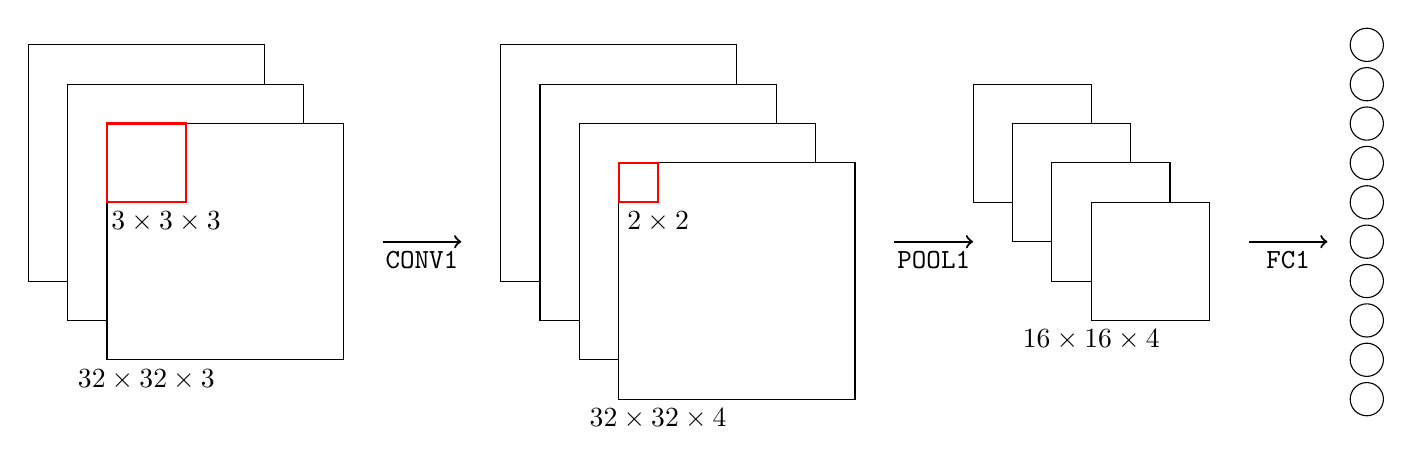
\begin{tikzpicture}
		\foreach \s in {0, ..., 2} {
			\draw [fill=white] (0.5*\s, -0.5*\s) rectangle (3 + 0.5*\s, -3 - 0.5*\s);
		}

		\node at (1.5, -4.25) {$32 \times 32 \times 3$};

		\draw [red, thick] (1, -1) rectangle (2, -2);
		\node at (1.75, -2.25) {$3 \times 3 \times 3$};

		\draw [->, thick] (4.5, -2.5) -- (5.5, -2.5) node [midway, below] {\texttt{CONV1}};

		\foreach \s in {0, ..., 3} {
			\draw [fill=white] (6 + 0.5*\s, -0.5*\s) rectangle (9 + 0.5*\s, -3 - 0.5*\s);
		}

		\node at (8, -4.75) {$32 \times 32 \times 4$};

		\draw [red, thick] (7.5, -1.5) rectangle (8, -2);
		\node at (8, -2.25) {$2 \times 2$};

		\draw [->, thick] (11, -2.5) -- (12, -2.5) node [midway, below] {\texttt{POOL1}};

		\foreach \s in {0, ..., 3} {
			\draw [fill=white] (12 + 0.5*\s, -0.5 - 0.5*\s) rectangle (13.5 + 0.5*\s, -2 - 0.5*\s);
		}

		\node at (13.5, -3.75) {$16 \times 16 \times 4$};

		\foreach \i in {0, ..., 9} {
			\draw (17, -0.5*\i) circle (6pt);
		}

		\draw [->, thick] (15.5, -2.5) -- (16.5, -2.5) node [midway, below] {\texttt{FC1}};
	\end{tikzpicture}}
	\caption{Our CNN architecture structure}
	\label{fig:cnn-structure}
\end{figure}
The TensorFlow implementations were trained using 12,800,000 samples using mini-batch stochastic gradient descent. We trained the model using Amazon EC2 spot instances with \code{c2x.large} (8-Core Xeon) and \code{c8x.large} (32-Core Xeon) processors.